\documentclass[9pt]{extarticle}
\usepackage[a4paper,landscape,margin=9mm]{geometry}
\usepackage[T1]{fontenc}
\usepackage{lmodern}
\usepackage{graphicx,xcolor,amsmath,amssymb}
\pagestyle{empty}
\setlength{\parindent}{0pt}
\definecolor{acc}{RGB}{20,60,120}
\definecolor{accl}{RGB}{235,240,250}
\newcommand{\secrule}[1]{{\large\bfseries\textcolor{acc}{#1}}\par\vspace{1pt}{\color{acc}\rule{\linewidth}{1.2pt}}\par\vspace{3pt}}
\newcommand{\doi}[1]{{\footnotesize\texttt{#1}}}
\begin{document}

% ===================== PAGE 1 =====================
\begin{minipage}[t]{\textwidth}
\colorbox{accl}{\begin{minipage}{0.992\textwidth}\vspace{2pt}
{\LARGE\bfseries Dual Geometry of Wavelength Space and Frequency Space}\quad{\large Series Handout, Papers 1--12}\\[2pt]
{\large From three assumptions: how much of what looks quantum and spacetime-like follows \emph{as theorems}?}\\[2pt]
Noriaki Kihara (WF System Co., Ltd.)\quad ORCID: 0009-0004-6753-4020 \quad CC BY 4.0 \quad June 2026 \quad All papers on Zenodo, bilingual (JA/EN)
\vspace{2pt}\end{minipage}}
\end{minipage}

\vspace{4pt}
\begin{minipage}[t]{0.30\textwidth}
\secrule{The Three Assumptions (entire inventory)}
\textbf{1.\ Reciprocal duality}\quad $\nu\lambda=1$\\
\textbf{2.\ Zero point}\quad $1/2$\\
\textbf{3.\ Asymmetric one bit}\quad the conservation law $\sum\nu^2$ rides only one side of the duality\\[3pt]
{\small Operating principles: configuration reading and the record principle. Continuous spacetime, amplitudes, wave functions, and collapse are \textbf{not assumed}.}

\vspace{5pt}
\secrule{Discipline of Method}
{\small An observational model: no identification with physical quantities. Every claim is backed by exhaustive enumeration, exact identities, or machine-precision numerics. Relations to standard theory are stated as \emph{structural correspondences}; every paper carries an explicit ``claims / non-claims'' section.}

\vspace{5pt}
\secrule{Foundations: Papers 1--4 (published)}
{\small
\textbf{Paper 1}\ Reciprocal duality, log representation, the 4D lattice count $N_0(R)$\ \doi{10.5281/zenodo.20588036}\\
\textbf{Paper 2}\ Exact tables for $R=0.5$--$10^4$ ($N_0=1,9,137,\ldots$)\ \doi{10.5281/zenodo.20588038}\\
\textbf{Paper 3}\ Supplement: connection to radial projection\ \doi{10.5281/zenodo.20589261}\\
\textbf{Paper 4}\ Splitting representation, volume gap, duality breaking, self-similar hierarchy\ \doi{10.5281/zenodo.20638962}
}
\end{minipage}\hfill
\begin{minipage}[t]{0.37\textwidth}
\secrule{The Twin Minimal Space Model (Paper 12)}
\begin{center}
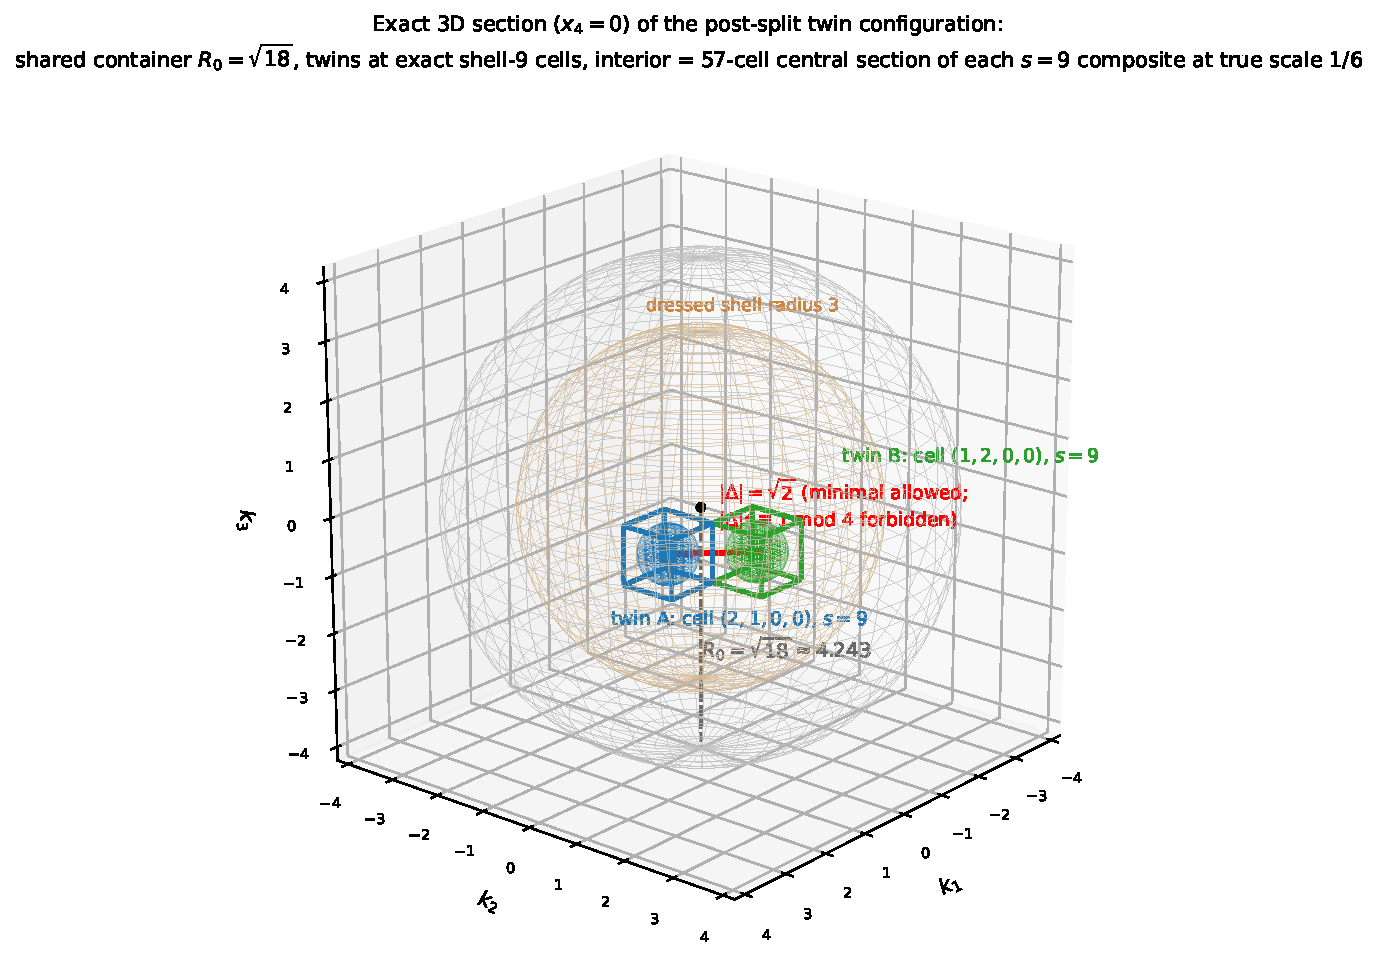
\includegraphics[height=58mm,keepaspectratio]{figure_paper12_2_twin_configuration.pdf}
\end{center}
{\footnotesize \textbf{Exact 3D section} ($x_4=0$) of the post-split twin configuration. Inside the shared container $R_0=\sqrt{18}$ the twins occupy actual shell-9 cells; the minimal allowed separation is $|\Delta|=\sqrt2$ ($|\Delta|^2\equiv1$ mod 4 forbidden). Each cell interior shows the 57-cube central section of the next-level 137-cell composite at true scale $1/6$ --- every position, separation, and scale is a computed value.}
\end{minipage}\hfill
\begin{minipage}[t]{0.30\textwidth}
\secrule{The Chain of Theorems (Papers 5$\to$12)}
{\footnotesize
\textbf{5\ Dictionary theorem}: lattice counting $=$ real standing-wave counting with zero point (exact). $R^2$ quantized to odd integers; the 137/105 issue resolved\\[2pt]
\textbf{6\ Freezing theorem}: the asymmetric bit \emph{is} the existence condition for time-like structure. Record theorem, null structure, invariant area\\[2pt]
\textbf{7\ Exclusion statistics derived}: stable species $\{1,3,5\}$, threshold $s=7$, unique branching $77.4\%:22.6\%$\\[2pt]
\textbf{8\ Accounting inverted}: shared curvature $\to$ condensation; internal expansion $a\propto t^{1/2}$; vacuum as an area reservoir\\[2pt]
\textbf{9\ Half-wavelength censorship}: shifts $\le\frac12$ (saturated exactly) protect composites; existence ceiling, forced hierarchization\\[2pt]
\textbf{10\ Emergent gauge}: kinematically unique connection, holonomy $\pi/2=$ geodesic area, SO(4) forced\\[2pt]
\textbf{11\ Dimension}: $d=4$ selected in a pincer --- censorship ceiling, mod 8, self-dual seed\\[2pt]
\textbf{12\ Twin model}: measurement $=$ append (absence$\to$presence), layer resolution of entanglement, hidden axes $R$/$Q$
}
\end{minipage}

\vspace{3pt}
\begin{minipage}[t]{0.64\textwidth}
\begin{center}
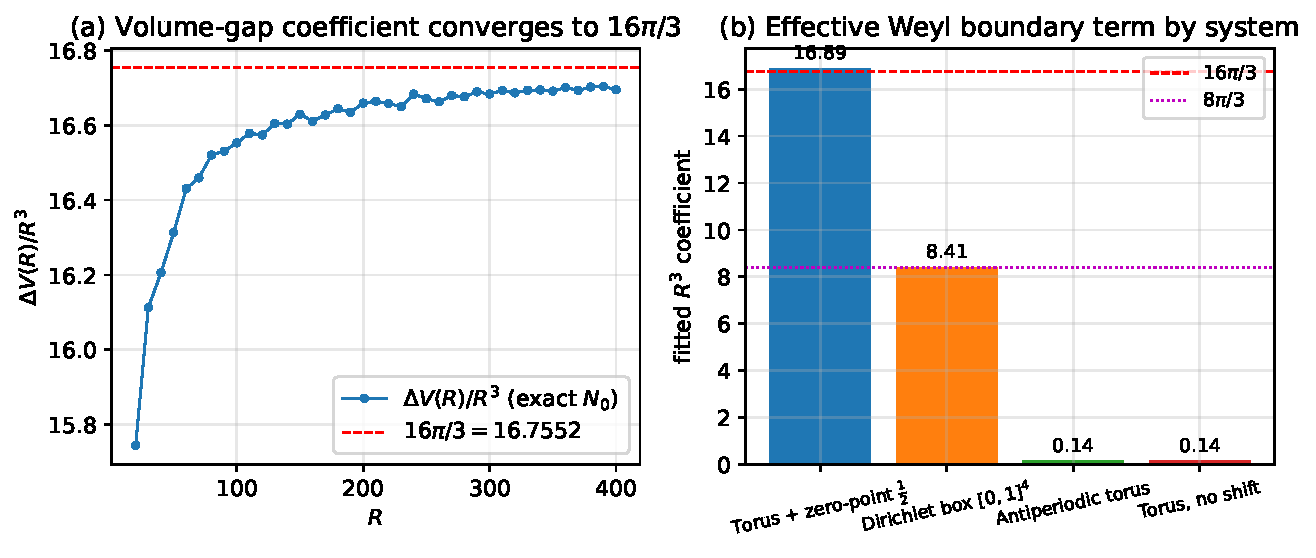
\includegraphics[height=36mm,keepaspectratio]{figure_paper5_1_weyl_gap_convergence.pdf}
\end{center}
\vspace{-4pt}
{\footnotesize \textbf{Verifying the dictionary (Paper 5)}: the volume-gap coefficient converges to $16\pi/3$ (left; exact $N_0$, $R\le400$). Right: four boundary systems --- the zero-point shift generates an effective Weyl boundary of \textbf{exactly twice} the Dirichlet unit box.}
\end{minipage}\hfill
\begin{minipage}[t]{0.33\textwidth}
\vspace{2pt}
\colorbox{accl}{\begin{minipage}{0.97\linewidth}\vspace{2pt}{\small
\textbf{The core sequence}\quad $N_0(R)=1,\ 9,\ 137,\ 473,\ 1545,\ \ldots$\\
Condition: $\sum_{i=1}^4(|k_i|+\tfrac12)^2\le R^2$\\[2pt]
Zero point $\tfrac12$ $\to$ cell $=$ standing wave $\to$ non-overlap $=$ orthogonality $\to$ odd-rule coherence $\to$ exception-free splitting $\to$ quantization of $R^2$ --- a chain with no added assumptions.}\vspace{2pt}\end{minipage}}
\end{minipage}

\newpage
% ===================== PAGE 2 =====================
\begin{minipage}[t]{0.64\textwidth}
\secrule{The Development: Papers 5--12 (v0.2, released 2026-06-11)}
{\small
\begin{tabular}{@{}p{0.30\linewidth}p{0.43\linewidth}p{0.22\linewidth}@{}}
\textbf{5}\ The Cell--Standing-Wave Dictionary & dictionary theorem, zero-point quantum, $16\pi/3$ as Weyl deficit, classification theorem & \doi{10.5281/zenodo.20640454}\\[2pt]
\textbf{6}\ Conservation, Records, Time-like Structure & freezing theorem, $B_4$ gauge, $1{+}3$ polar split, record theorem & \doi{10.5281/zenodo.20640456}\\[2pt]
\textbf{7}\ Configuration Statistics \& Relational Readout & exclusion statistics, stable species, branching ratios, holographic readout & \doi{10.5281/zenodo.20640458}\\[2pt]
\textbf{8}\ Two Accountings & optimality of condensation, Jeans-type threshold, $a\propto t^{1/2}$, area law & \doi{10.5281/zenodo.20640460}\\[2pt]
\textbf{9}\ Logic Waves \& Half-Wavelength Censorship & amplitude-free coherence, kinematic stabilization, three-band structure & \doi{10.5281/zenodo.20640462}\\[2pt]
\textbf{10}\ Emergent Gauge Structure & holonomy $\pi/2$, SO(4) forced, spin lift, $\beta=0$ & \doi{10.5281/zenodo.20640464}\\[2pt]
\textbf{11}\ The Necessity of Dimension & both-endpoint theorem $[0,4]$, mod 8, four-legs theorem, self-dual seed & \doi{10.5281/zenodo.20640466}\\[2pt]
\textbf{12}\ The Twin Minimal Space Model & measurement as append, measure bifurcation, no-signaling, licensed virtual displacements & \doi{10.5281/zenodo.20640468}\\
\end{tabular}}
\end{minipage}\hfill
\begin{minipage}[t]{0.33\textwidth}
\secrule{Highlights}
{\small
\textbf{Two-tier agreement}: stable species $\{1,3,5\}$ and threshold $s=7$ reached by \textbf{independent computations} --- counting (Paper 7) and waves (Paper 9)\\[2pt]
\textbf{Fewer postulates}: exclusion, collapse, the arrow of time, and the integer lattice move from assumptions to theorems / resolution structure\\[2pt]
\textbf{Falsifiability}: amplitudes cannot couple to curvature (Paper 9) --- BMV-type gravitationally mediated entanglement experiments are a live referee\\[2pt]
\textbf{Not re-deriving is not a defect}: the transport principle (Paper 12). The difference lies in candidate answers to questions standard theory leaves as postulates (collapse, the cut, time, dimension)}
\end{minipage}

\vspace{6pt}
\begin{minipage}[t]{0.40\textwidth}
\begin{center}
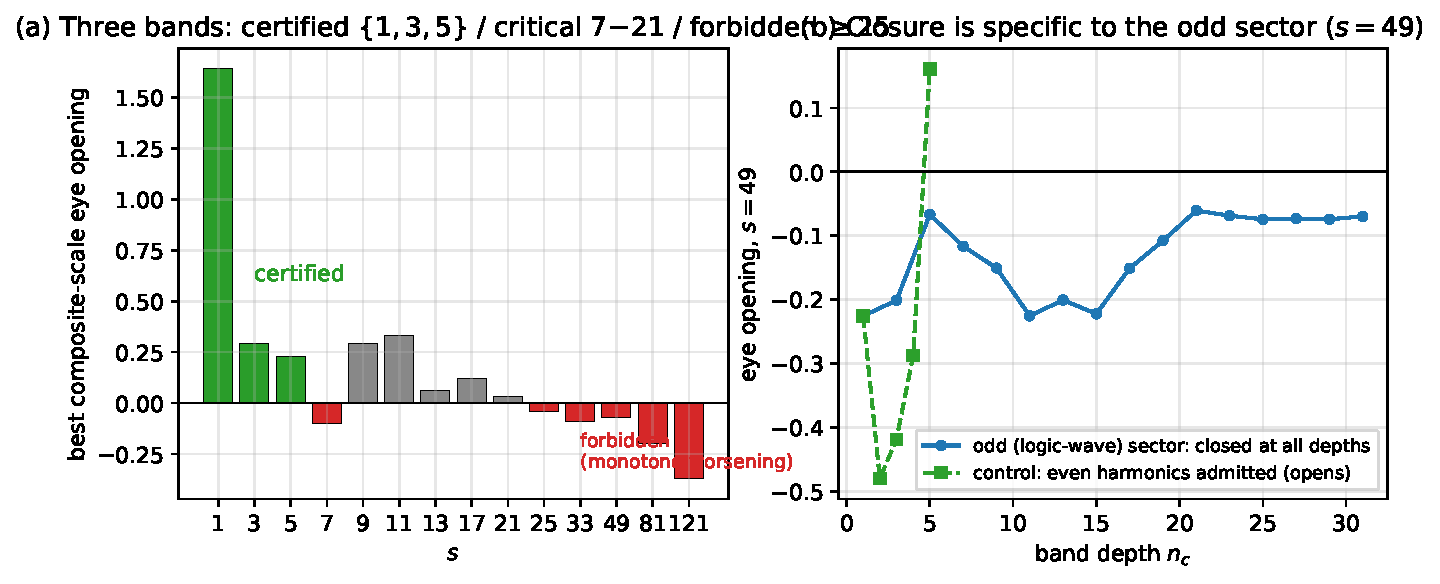
\includegraphics[height=42mm,keepaspectratio]{figure_paper9_3_three_bands.pdf}
\end{center}
\vspace{-4pt}
{\small \textbf{Three bands of existence (Paper 9)}: self-certification margins split into certified $\{1,3,5\}$ / critical / forbidden ($s\ge25$); for $s\ge49$ the whole odd sector closes (right). Admitting even harmonics reopens it --- closure is specific to logic waves.}
\end{minipage}\hfill
\begin{minipage}[t]{0.29\textwidth}
\begin{center}
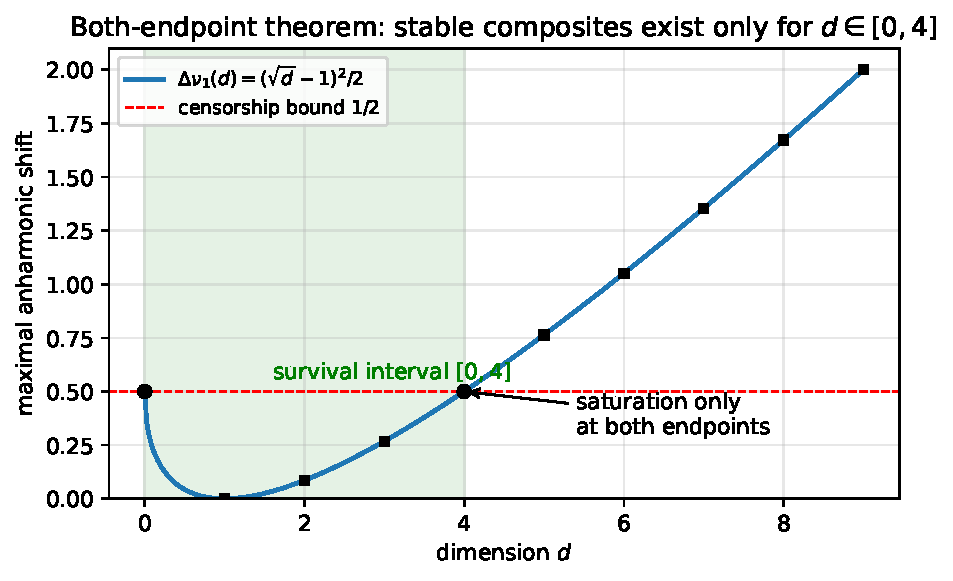
\includegraphics[height=42mm,keepaspectratio]{figure_paper11_1_survival_interval.pdf}
\end{center}
\vspace{-4pt}
{\small \textbf{Both-endpoint theorem (Paper 11)}: $\Delta\nu_1(d)=(\sqrt d-1)^2/2\le\frac12 \iff d\in[0,4]$, saturated only at the endpoints --- $d=4$ is critical at the ceiling.}
\end{minipage}\hfill
\begin{minipage}[t]{0.27\textwidth}
\begin{center}
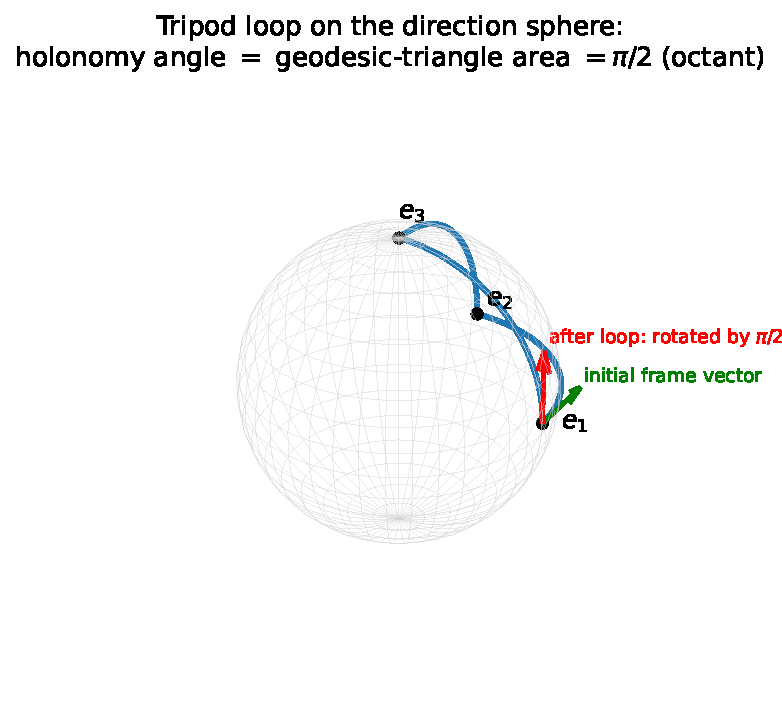
\includegraphics[height=50mm,keepaspectratio]{figure_paper10_1_tripod_holonomy.pdf}
\end{center}
\vspace{-4pt}
{\small \textbf{The first holonomy (Paper 10)}: transport around the tripod loop rotates by $\pi/2$ --- exactly the area of the geodesic octant. Discrete transport reproduces continuous curvature.}
\end{minipage}

\vspace{5pt}
{\color{acc}\rule{\textwidth}{1.2pt}}\\[2pt]
{\small \textbf{Research notes (Supplements 1--41), all verification scripts, and figure-generation code}: \texttt{github.com/WurabeSeiji/ai-chat-logs-open} (folder ``Dual Geometry of Wavelength Space and Frequency Space'').\quad
All figures are exact computations (no schematic diagrams). This series is an observational model; it does not claim to derive or modify physical theory.}

\end{document}
